In questo capitolo analizzeremo i risultati ottenuti dall'applicazione della metodologia proposta ai dataset considerati e ai risultati ottenuti dall'inferenza del modello. Verranno presentati i principali indicatori di performance, le metriche di valutazione del drift e le eventuali osservazioni emerse durante l'analisi dei dati.
\section{Analisi delle metriche di drift sui dataset}
Per analizzare l'avvenimento di un data drift rispetto ad imagenet-1k, ci avvarremo di un test statistico (Distanza di Wesserstein) sulle seguenti misure:
\begin{itemize}
	\item Luminanza
	\item Contrasto
	\item Nitidezza (Sharpness)
	\item Media dei canali colore
\end{itemize}
\subsection{ImageNet-1k vs ImageNet-R}
Come si può evincere dal grafico in figura \ref{fig:imagenet_r_drift_image}, la maggior parte delle feature presenta un drift rispetto alla distribuzione di riferimento (imagenet-1k) secondo la distanza di Wesserstein.
In particolare, tutte le misure tranne sharpness presentano un drift significativo, con valori di distanza di Wesserstein superiori a 0.1. La misura di sharpness, invece, risulta essere più simile alla distribuzione di riferimento, con un valore di distanza di Wesserstein inferiore a 0.1. Possiamo inoltre osservare che la distribuzione di brightness presenta una distanza di Wesserstein molto maggiore dei canali colore. Questo potrebbe essere dovuto al fatto che essendo ImageNet-R formato da immagini artistiche, tra cui disegni è possibile che ci sia un maggior numero d'immagini con uno sfondo bianco, dunque una maggiore varianza nella luminosità.
\begin{figure}
	\centering
	
\includegraphics[width=\textwidth]{images/metrics/ImageNet-R/drift_distr_imagenet-1k_vs_imagenet-r.png}
	\caption{Distribuzione delle misure di luminanza, contrasto, nitidezza e media dei canali colore per ImageNet-1k e ImageNet-R.}
	\label{fig:imagenet_r_drift_image}
\end{figure}
\subsection{ImageNet-1k vs ImageNet-C}
Per quanto riguarda ImageNet-C, abbiamo osservato i risultati distinguendo le corruzioni per tipo di corruzione e severità (1-5).
\newcommand{\driftcell}[1]{%
  \ifdim #1pt < 0.1pt
    \textcolor{green!60!black}{#1}%
  \else
    \textcolor{red!75!black}{#1}%
  \fi
}
% noise
\begin{table}[H]
	\centering
	\label{tab:imagenet_c_drift_metrics_noise}
\begin{tabular}{llrrrrr}
\toprule
corruption & feature & sev\_1 & sev\_2 & sev\_3 & sev\_4 & sev\_5 \\
\midrule
gaussian\_noise & brightness & \driftcell{0.072713} & \driftcell{0.085192} & \driftcell{0.112507} & \driftcell{0.162998} & \driftcell{0.251874} \\
gaussian\_noise & mean\_blue & \driftcell{0.028428} & \driftcell{0.040312} & \driftcell{0.083820} & \driftcell{0.159918} & \driftcell{0.274003} \\
gaussian\_noise & mean\_green & \driftcell{0.053796} & \driftcell{0.065129} & \driftcell{0.086815} & \driftcell{0.128471} & \driftcell{0.203225} \\
gaussian\_noise & mean\_red & \driftcell{0.046630} & \driftcell{0.043086} & \driftcell{0.060681} & \driftcell{0.122065} & \driftcell{0.223818} \\
gaussian\_noise & rms\_contrast & \driftcell{0.114575} & \driftcell{0.126554} & \driftcell{0.220013} & \driftcell{0.380643} & \driftcell{0.601419} \\
gaussian\_noise & sharpness & \driftcell{1.385858} & \driftcell{2.396271} & \driftcell{3.420685} & \driftcell{4.200996} & \driftcell{4.791838} \\
impulse\_noise & brightness & \driftcell{0.080418} & \driftcell{0.103368} & \driftcell{0.126473} & \driftcell{0.189028} & \driftcell{0.267379} \\
impulse\_noise & mean\_blue & \driftcell{0.029314} & \driftcell{0.061542} & \driftcell{0.096882} & \driftcell{0.185154} & \driftcell{0.284710} \\
impulse\_noise & mean\_green & \driftcell{0.058434} & \driftcell{0.074756} & \driftcell{0.091807} & \driftcell{0.144506} & \driftcell{0.209471} \\
impulse\_noise & mean\_red & \driftcell{0.038153} & \driftcell{0.044674} & \driftcell{0.068579} & \driftcell{0.144231} & \driftcell{0.233162} \\
impulse\_noise & rms\_contrast & \driftcell{0.116605} & \driftcell{0.132207} & \driftcell{0.172549} & \driftcell{0.310412} & \driftcell{0.488980} \\
impulse\_noise & sharpness & \driftcell{0.857158} & \driftcell{1.551392} & \driftcell{2.150133} & \driftcell{3.356574} & \driftcell{4.291620} \\
shot\_noise & brightness & \driftcell{0.073568} & \driftcell{0.092625} & \driftcell{0.129523} & \driftcell{0.226492} & \driftcell{0.337091} \\
shot\_noise & mean\_blue & \driftcell{0.031541} & \driftcell{0.028833} & \driftcell{0.031633} & \driftcell{0.075767} & \driftcell{0.125525} \\
shot\_noise & mean\_green & \driftcell{0.038060} & \driftcell{0.035835} & \driftcell{0.035784} & \driftcell{0.056486} & \driftcell{0.089558} \\
shot\_noise & mean\_red & \driftcell{0.050125} & \driftcell{0.043082} & \driftcell{0.034105} & \driftcell{0.055221} & \driftcell{0.094603} \\
shot\_noise & rms\_contrast & \driftcell{0.106031} & \driftcell{0.139771} & \driftcell{0.253508} & \driftcell{0.506550} & \driftcell{0.723193} \\
shot\_noise & sharpness & \driftcell{1.504179} & \driftcell{2.558167} & \driftcell{3.451343} & \driftcell{4.334384} & \driftcell{4.723952} \\
\bottomrule
\end{tabular}
\caption{Distanza di Wesserstein tra le distribuzioni delle misure di luminanza, contrasto, nitidezza e media dei canali colore per ImageNet-C nel gruppo di corruzione noise.}
\end{table}
Possiamo notare dai dati nella tabella \ref{tab:imagenet_c_drift_metrics_noise} che per tutti i tipi di rumore le feature rms\_contrast e sharpness driftano a tutti i livelli di severità, mentre le altre feature driftano solo a severità più alte. In particolare, la feature sharpness presenta un drift molto più marcato rispetto alle altre feature, con valori di distanza di Wesserstein che superano 4 per la severità 5. Questo, può essere casuato dal fatto che il rumore può coprire i bordi degli oggetti. Possiamo notare inoltre che mean\_green e mean\_red per shot\_noise non driftano, mentre mean\_blue drifta solo al livello di severity 5.
Osservando la figura \ref{fig:imagenet_c_drift_severity_noise} possiamo notare che per noise la distanza nei canali colore non aumenta sempre all'aumentare della severità, questa diminuisce da severity 1 a severity 3. La distanza nelle altre feature aumenta invece sempre per tutti i rumori all'aumentare della severità. 
\begin{figure}[H]
	\centering
	
\includegraphics[width=\textwidth]{images/metrics/ImageNet-C/severity_curves/imagenet_c_severity_drift_noise.png}
	\caption{Distanza di Wesserstein tra le distribuzioni delle misure di luminanza, contrasto, nitidezza e media dei canali colore per ImageNet-C nel gruppo di corruzione noise, al variare della severità.}
	\label{fig:imagenet_c_drift_severity_noise}
\end{figure}
% blur
\begin{table}[H]
	\centering
	\label{tab:imagenet_c_drift_metrics_blur}
\begin{tabular}{llrrrrr}
\toprule
corruption & feature & sev\_1 & sev\_2 & sev\_3 & sev\_4 & sev\_5 \\
\midrule
defocus\_blur & brightness & \driftcell{0.060605} & \driftcell{0.060416} & \driftcell{0.060385} & \driftcell{0.050140} & \driftcell{0.049462} \\
defocus\_blur & mean\_blue & \driftcell{0.038377} & \driftcell{0.038431} & \driftcell{0.038553} & \driftcell{0.038591} & \driftcell{0.038571} \\
defocus\_blur & mean\_green & \driftcell{0.040674} & \driftcell{0.040607} & \driftcell{0.040626} & \driftcell{0.040581} & \driftcell{0.040763} \\
defocus\_blur & mean\_red & \driftcell{0.059018} & \driftcell{0.059035} & \driftcell{0.059161} & \driftcell{0.059179} & \driftcell{0.059252} \\
defocus\_blur & rms\_contrast & \driftcell{0.417192} & \driftcell{0.486428} & \driftcell{0.606822} & \driftcell{0.669142} & \driftcell{0.772384} \\
defocus\_blur & sharpness & \driftcell{1.265309} & \driftcell{1.283204} & \driftcell{1.292588} & \driftcell{1.292072} & \driftcell{1.294569} \\
glass\_blur & brightness & \driftcell{0.064491} & \driftcell{0.064835} & \driftcell{0.062973} & \driftcell{0.063866} & \driftcell{0.063666} \\
glass\_blur & mean\_blue & \driftcell{0.040414} & \driftcell{0.041017} & \driftcell{0.039830} & \driftcell{0.040450} & \driftcell{0.040463} \\
glass\_blur & mean\_green & \driftcell{0.040329} & \driftcell{0.040112} & \driftcell{0.039959} & \driftcell{0.039883} & \driftcell{0.039657} \\
glass\_blur & mean\_red & \driftcell{0.060777} & \driftcell{0.061247} & \driftcell{0.060013} & \driftcell{0.060569} & \driftcell{0.060458} \\
glass\_blur & rms\_contrast & \driftcell{0.350142} & \driftcell{0.423292} & \driftcell{0.497461} & \driftcell{0.569429} & \driftcell{0.691295} \\
glass\_blur & sharpness & \driftcell{1.158576} & \driftcell{1.232642} & \driftcell{1.238898} & \driftcell{1.258086} & \driftcell{1.286698} \\
motion\_blur & brightness & \driftcell{0.056901} & \driftcell{0.056778} & \driftcell{0.056420} & \driftcell{0.055830} & \driftcell{0.054923} \\
motion\_blur & mean\_blue & \driftcell{0.034105} & \driftcell{0.034367} & \driftcell{0.034439} & \driftcell{0.034397} & \driftcell{0.034168} \\
motion\_blur & mean\_green & \driftcell{0.041566} & \driftcell{0.041327} & \driftcell{0.041100} & \driftcell{0.040844} & \driftcell{0.040585} \\
motion\_blur & mean\_red & \driftcell{0.055418} & \driftcell{0.055543} & \driftcell{0.055489} & \driftcell{0.055315} & \driftcell{0.054954} \\
motion\_blur & rms\_contrast & \driftcell{0.344950} & \driftcell{0.438142} & \driftcell{0.551789} & \driftcell{0.662401} & \driftcell{0.744262} \\
motion\_blur & sharpness & \driftcell{1.041598} & \driftcell{1.140697} & \driftcell{1.199950} & \driftcell{1.232650} & \driftcell{1.247467} \\
zoom\_blur & brightness & \driftcell{0.066676} & \driftcell{0.068524} & \driftcell{0.070336} & \driftcell{0.071692} & \driftcell{0.073191} \\
zoom\_blur & mean\_blue & \driftcell{0.043693} & \driftcell{0.045843} & \driftcell{0.047872} & \driftcell{0.049723} & \driftcell{0.051801} \\
zoom\_blur & mean\_green & \driftcell{0.049571} & \driftcell{0.052709} & \driftcell{0.055854} & \driftcell{0.058789} & \driftcell{0.062629} \\
zoom\_blur & mean\_red & \driftcell{0.068991} & \driftcell{0.072782} & \driftcell{0.076475} & \driftcell{0.079874} & \driftcell{0.083973} \\
zoom\_blur & rms\_contrast & \driftcell{0.458881} & \driftcell{0.526616} & \driftcell{0.611801} & \driftcell{0.661374} & \driftcell{0.740796} \\
zoom\_blur & sharpness & \driftcell{1.165725} & \driftcell{1.206743} & \driftcell{1.218080} & \driftcell{1.235984} & \driftcell{1.237147} \\
\bottomrule
\end{tabular}
\caption{Distanza di Wesserstein tra le distribuzioni delle misure di luminanza, contrasto, nitidezza e media dei canali colore per ImageNet-C nel gruppo di corruzione blur.}
\end{table}
Possiamo notare dai dati in tabella \ref{tab:imagenet_c_drift_metrics_blur} che per tutti i tipi di blur la brightness e i canali colore non driftano, questo accade perché i blur non modificano la luminosità o i colori delle immagini. Le feature rms\_contrast e sharpness driftano a tutti i livelli di severità. In particolare, la feature sharpness presenta un drift molto più marcato rispetto alle altre feature, con valori di distanza di Wesserstein che superano 1.2 per la severità 5. Questo, può essere causato dal fatto che il blur può coprire i bordi degli oggetti, diminuendo la nitidezza e il contrasto, come si può osservare ad esempio nella figura \ref{fig:imagenet_c_drift_image_glass}. Come si può notare inoltre dalla figura \ref{fig:imagenet_c_drift_severity_blur}, le feature che non presentano drift hanno un andamento pressoché costante per ogni livello di severità, tranne per zoom\_blur, il quale andamento è quasi lineare all'aumentare del livello di severità. Inoltre, i valori della distanza di Wesserstein per sharpness sono molto vicini fra loro per ogni livello di severità e tipo di blur.
\begin{figure}[H]
	\centering
	
\includegraphics[width=\textwidth]{images/metrics/ImageNet-C/severity_curves/imagenet_c_severity_drift_blur.png}
	\caption{Distanza di Wesserstein tra le distribuzioni delle misure di luminanza, contrasto, nitidezza e media dei canali colore per ImageNet-C nel gruppo di corruzione blur, al variare della severità.}
	\label{fig:imagenet_c_drift_severity_blur}
\end{figure}
% weather
\begin{table}[H]
	\centering
	\label{tab:imagenet_c_drift_metrics_weather}
\begin{tabular}{llrrrrr}
\toprule
corruption & feature & sev\_1 & sev\_2 & sev\_3 & sev\_4 & sev\_5 \\
\midrule
brightness & brightness & \driftcell{0.576325} & \driftcell{1.128612} & \driftcell{1.609895} & \driftcell{2.022776} & \driftcell{2.348483} \\
brightness & mean\_blue & \driftcell{0.037699} & \driftcell{0.043582} & \driftcell{0.047753} & \driftcell{0.053588} & \driftcell{0.056299} \\
brightness & mean\_green & \driftcell{0.039589} & \driftcell{0.040811} & \driftcell{0.042565} & \driftcell{0.052990} & \driftcell{0.059364} \\
brightness & mean\_red & \driftcell{0.057856} & \driftcell{0.063008} & \driftcell{0.064307} & \driftcell{0.068695} & \driftcell{0.069323} \\
brightness & rms\_contrast & \driftcell{0.194603} & \driftcell{0.343004} & \driftcell{0.586194} & \driftcell{0.913852} & \driftcell{1.269411} \\
brightness & sharpness & \driftcell{0.239242} & \driftcell{0.248618} & \driftcell{0.285387} & \driftcell{0.348412} & \driftcell{0.429741} \\
fog & brightness & \driftcell{0.337783} & \driftcell{0.344840} & \driftcell{0.364152} & \driftcell{0.401109} & \driftcell{0.441012} \\
fog & mean\_blue & \driftcell{0.525600} & \driftcell{0.576151} & \driftcell{0.612098} & \driftcell{0.613082} & \driftcell{0.639908} \\
fog & mean\_green & \driftcell{0.380592} & \driftcell{0.415061} & \driftcell{0.439368} & \driftcell{0.440063} & \driftcell{0.458478} \\
fog & mean\_red & \driftcell{0.457440} & \driftcell{0.503187} & \driftcell{0.535868} & \driftcell{0.536735} & \driftcell{0.561158} \\
fog & rms\_contrast & \driftcell{1.694664} & \driftcell{1.723715} & \driftcell{1.590665} & \driftcell{1.471921} & \driftcell{1.383768} \\
fog & sharpness & \driftcell{1.103313} & \driftcell{1.169476} & \driftcell{1.208260} & \driftcell{1.207460} & \driftcell{1.229185} \\
frost & brightness & \driftcell{1.681603} & \driftcell{1.974560} & \driftcell{2.112238} & \driftcell{1.987928} & \driftcell{2.055561} \\
frost & mean\_blue & \driftcell{0.469288} & \driftcell{0.643080} & \driftcell{0.722371} & \driftcell{0.743677} & \driftcell{0.783210} \\
frost & mean\_green & \driftcell{0.212773} & \driftcell{0.240710} & \driftcell{0.249700} & \driftcell{0.248716} & \driftcell{0.254829} \\
frost & mean\_red & \driftcell{0.436628} & \driftcell{0.609805} & \driftcell{0.691184} & \driftcell{0.713028} & \driftcell{0.753416} \\
frost & rms\_contrast & \driftcell{0.537042} & \driftcell{1.067577} & \driftcell{1.318931} & \driftcell{1.377810} & \driftcell{1.495522} \\
frost & sharpness & \driftcell{0.285483} & \driftcell{0.293777} & \driftcell{0.247972} & \driftcell{0.242873} & \driftcell{0.210797} \\
snow & brightness & \driftcell{1.146456} & \driftcell{1.850992} & \driftcell{1.839177} & \driftcell{2.211917} & \driftcell{2.592699} \\
snow & mean\_blue & \driftcell{0.373648} & \driftcell{0.528322} & \driftcell{0.529197} & \driftcell{0.599734} & \driftcell{0.670009} \\
snow & mean\_green & \driftcell{0.269782} & \driftcell{0.371856} & \driftcell{0.373095} & \driftcell{0.420665} & \driftcell{0.467768} \\
snow & mean\_red & \driftcell{0.322548} & \driftcell{0.463436} & \driftcell{0.463859} & \driftcell{0.526932} & \driftcell{0.588320} \\
snow & rms\_contrast & \driftcell{0.099864} & \driftcell{0.189850} & \driftcell{0.176810} & \driftcell{0.226027} & \driftcell{0.652584} \\
snow & sharpness & \driftcell{0.461836} & \driftcell{1.037702} & \driftcell{0.549788} & \driftcell{0.515835} & \driftcell{0.599181} \\
\bottomrule
\end{tabular}
\caption{Distanza di Wesserstein tra le distribuzioni delle misure di luminanza, contrasto, nitidezza e media dei canali colore per ImageNet-C nel gruppo di corruzione weather.}
\end{table}
Come si può notare dalla tabella \ref{tab:imagenet_c_drift_metrics_weather}, per il tipo di sporcatura brightness, i valori medi dei canali colore non presentano drift, poiché modificare la luminosità non comporta una modifica nel colore dell'immagine, mentre le feature brightness, rms\_contrast e sharpness invece presentano un drift rispetto alla distribuzione di confronto. Infatti, come si può notare dall'immagine \ref{fig:imagenet_c_drift_image_brightness} aumentando la luminosità dell'immagine, oltre ovviamente ad introdurre un drift nella distribuzione della feature brightness, la feature
contrast presenta una diminuzione dei suoi valori mentre la feature sharpness presenta una minore concentrazione nelle code della distribuzione, mentre aumenta la frequenza dei valori pù frequenti, portando le distribuzioni a schiacciarsi. Questo può essere dal fatto che aumentare la luminosità di un'immagine la porta ad essere più tendente al bianco, quindi diminuendo
il contrasto e mediamente diminuendo la sua nitidezza. Possiamo inoltre fare le seguenti affermazioni riguardanti la figura \ref{fig:imagenet_c_drift_severity_weather}:
\begin{itemize}
  \item La distanza di Wesserstein per le immagini sporcate con corruzione snow ha un picco con severity 2 per la feature sharpness. Infatti, come si può notare dall'immagine \ref{fig:imagenet_c_drift_image_snow}, 
  i valori di sharpness per severity 2 sono molto più alti rispetto alla distribuzione originale
  e alle distribuzioni delle altre severity. Questo può essere dato dal fatto che aumentando il numero di oggetti nell'immagine senza però andandola a coprire del tutto, i valori della nitidezza aumentano poiché anche gli elementi introdotti dalla sporcatura hanno bordi ben definiti. 
  \item La distanza di Wesserstein per le immagini sporcate con corruzione fog diminuisce dalla severity 2 in poi per la feature rms\_contrast. Come si può infatti notare dalla figura \ref{fig:imagenet_c_drift_image_fog}, la distribuzione di rms\_contrast per le
  immagini sporcate presentano una minore variabilità e si concentrano su minori valori di contrasto. Questo può essere dato dal fatto che applicando questo tipo di sporcatura, le immagini tendono verso una colorazione grigia uniforme, come si può anche notare dalle distribuzioni dei canali colore.
\end{itemize}

\begin{figure}[H]
	\centering
	
\includegraphics[width=\textwidth]{images/metrics/ImageNet-C/severity_curves/imagenet_c_severity_drift_weather.png}
	\caption{Distanza di Wesserstein tra le distribuzioni delle misure di luminanza, contrasto, nitidezza e media dei canali colore per ImageNet-C nel gruppo di corruzione weather, al variare della severità.}
	\label{fig:imagenet_c_drift_severity_weather}
\end{figure}
% digital
\begin{table}[H]
	\centering
	\label{tab:imagenet_c_drift_metrics_digital}
\begin{tabular}{llrrrrr}
\toprule
corruption & feature & sev\_1 & sev\_2 & sev\_3 & sev\_4 & sev\_5 \\
\midrule
contrast & brightness & \driftcell{0.060245} & \driftcell{0.060239} & \driftcell{0.060229} & \driftcell{0.060227} & \driftcell{0.060195} \\
contrast & mean\_blue & \driftcell{0.038418} & \driftcell{0.038245} & \driftcell{0.037904} & \driftcell{0.037598} & \driftcell{0.037547} \\
contrast & mean\_green & \driftcell{0.041440} & \driftcell{0.041902} & \driftcell{0.042790} & \driftcell{0.043391} & \driftcell{0.043403} \\
contrast & mean\_red & \driftcell{0.059435} & \driftcell{0.059512} & \driftcell{0.059563} & \driftcell{0.059451} & \driftcell{0.059261} \\
contrast & rms\_contrast & \driftcell{2.330083} & \driftcell{2.691652} & \driftcell{3.053031} & \driftcell{3.413698} & \driftcell{3.593123} \\
contrast & sharpness & \driftcell{1.112014} & \driftcell{1.212285} & \driftcell{1.281598} & \driftcell{1.318082} & \driftcell{1.325120} \\
elastic\_transform & brightness & \driftcell{0.051794} & \driftcell{0.044459} & \driftcell{0.059603} & \driftcell{0.059610} & \driftcell{0.059654} \\
elastic\_transform & mean\_blue & \driftcell{0.039154} & \driftcell{0.042950} & \driftcell{0.036830} & \driftcell{0.036657} & \driftcell{0.036251} \\
elastic\_transform & mean\_green & \driftcell{0.043501} & \driftcell{0.049631} & \driftcell{0.041769} & \driftcell{0.041790} & \driftcell{0.042117} \\
elastic\_transform & mean\_red & \driftcell{0.061286} & \driftcell{0.067652} & \driftcell{0.058096} & \driftcell{0.057926} & \driftcell{0.057702} \\
elastic\_transform & rms\_contrast & \driftcell{0.269896} & \driftcell{0.304468} & \driftcell{0.249420} & \driftcell{0.249590} & \driftcell{0.249708} \\
elastic\_transform & sharpness & \driftcell{0.862587} & \driftcell{0.768063} & \driftcell{0.821826} & \driftcell{0.774113} & \driftcell{0.614177} \\
jpeg\_compression & brightness & \driftcell{0.057809} & \driftcell{0.057875} & \driftcell{0.058283} & \driftcell{0.058583} & \driftcell{0.057985} \\
jpeg\_compression & mean\_blue & \driftcell{0.022065} & \driftcell{0.026881} & \driftcell{0.018877} & \driftcell{0.021624} & \driftcell{0.023145} \\
jpeg\_compression & mean\_green & \driftcell{0.060105} & \driftcell{0.051337} & \driftcell{0.057659} & \driftcell{0.054069} & \driftcell{0.058407} \\
jpeg\_compression & mean\_red & \driftcell{0.052134} & \driftcell{0.051353} & \driftcell{0.046059} & \driftcell{0.043821} & \driftcell{0.035850} \\
jpeg\_compression & rms\_contrast & \driftcell{0.183292} & \driftcell{0.187883} & \driftcell{0.190634} & \driftcell{0.196080} & \driftcell{0.196912} \\
jpeg\_compression & sharpness & \driftcell{0.469067} & \driftcell{0.514780} & \driftcell{0.534496} & \driftcell{0.564141} & \driftcell{0.578935} \\
pixelate & brightness & \driftcell{0.056300} & \driftcell{0.056056} & \driftcell{0.056462} & \driftcell{0.056612} & \driftcell{0.056343} \\
pixelate & mean\_blue & \driftcell{0.029980} & \driftcell{0.029781} & \driftcell{0.031634} & \driftcell{0.032457} & \driftcell{0.032972} \\
pixelate & mean\_green & \driftcell{0.043141} & \driftcell{0.042790} & \driftcell{0.042617} & \driftcell{0.042332} & \driftcell{0.041621} \\
pixelate & mean\_red & \driftcell{0.052299} & \driftcell{0.051931} & \driftcell{0.053595} & \driftcell{0.054230} & \driftcell{0.054373} \\
pixelate & rms\_contrast & \driftcell{0.223815} & \driftcell{0.236370} & \driftcell{0.276135} & \driftcell{0.321615} & \driftcell{0.353021} \\
pixelate & sharpness & \driftcell{0.318243} & \driftcell{0.342908} & \driftcell{0.411007} & \driftcell{0.488771} & \driftcell{0.533425} \\
\bottomrule
\end{tabular}
\caption{Distanza di Wesserstein tra le distribuzioni delle misure di luminanza, contrasto, nitidezza e media dei canali colore per ImageNet-C nel gruppo di corruzione digital.}
Come si può notare dalla tabella \ref{tab:imagenet_c_drift_metrics_digital}, le uniche feature che presentano un drift secondo la distanza di Wesserstein sono il contrasto e la nitidezza. In particolare possiamo compiere le seguenti osservazioni:
\begin{itemize}
  \item Nonostante venga modificato direttamente il contrasto dell'immagini nel tipo di sporcatura contrast, la media dei canali colori non presenta drift in nessun livello di severità. Infatti, come si può osservare nella figura \ref{fig:imagenet_c_drift_image_contrast}, nonostante il contrasto venga diminuito rendendo l'immagine più uniforme a livello di colore, il valore medio dei canali colore rimane sostanzialmente invariato. 
\end{itemize}
\end{table}
\begin{figure}[H]
	\centering
	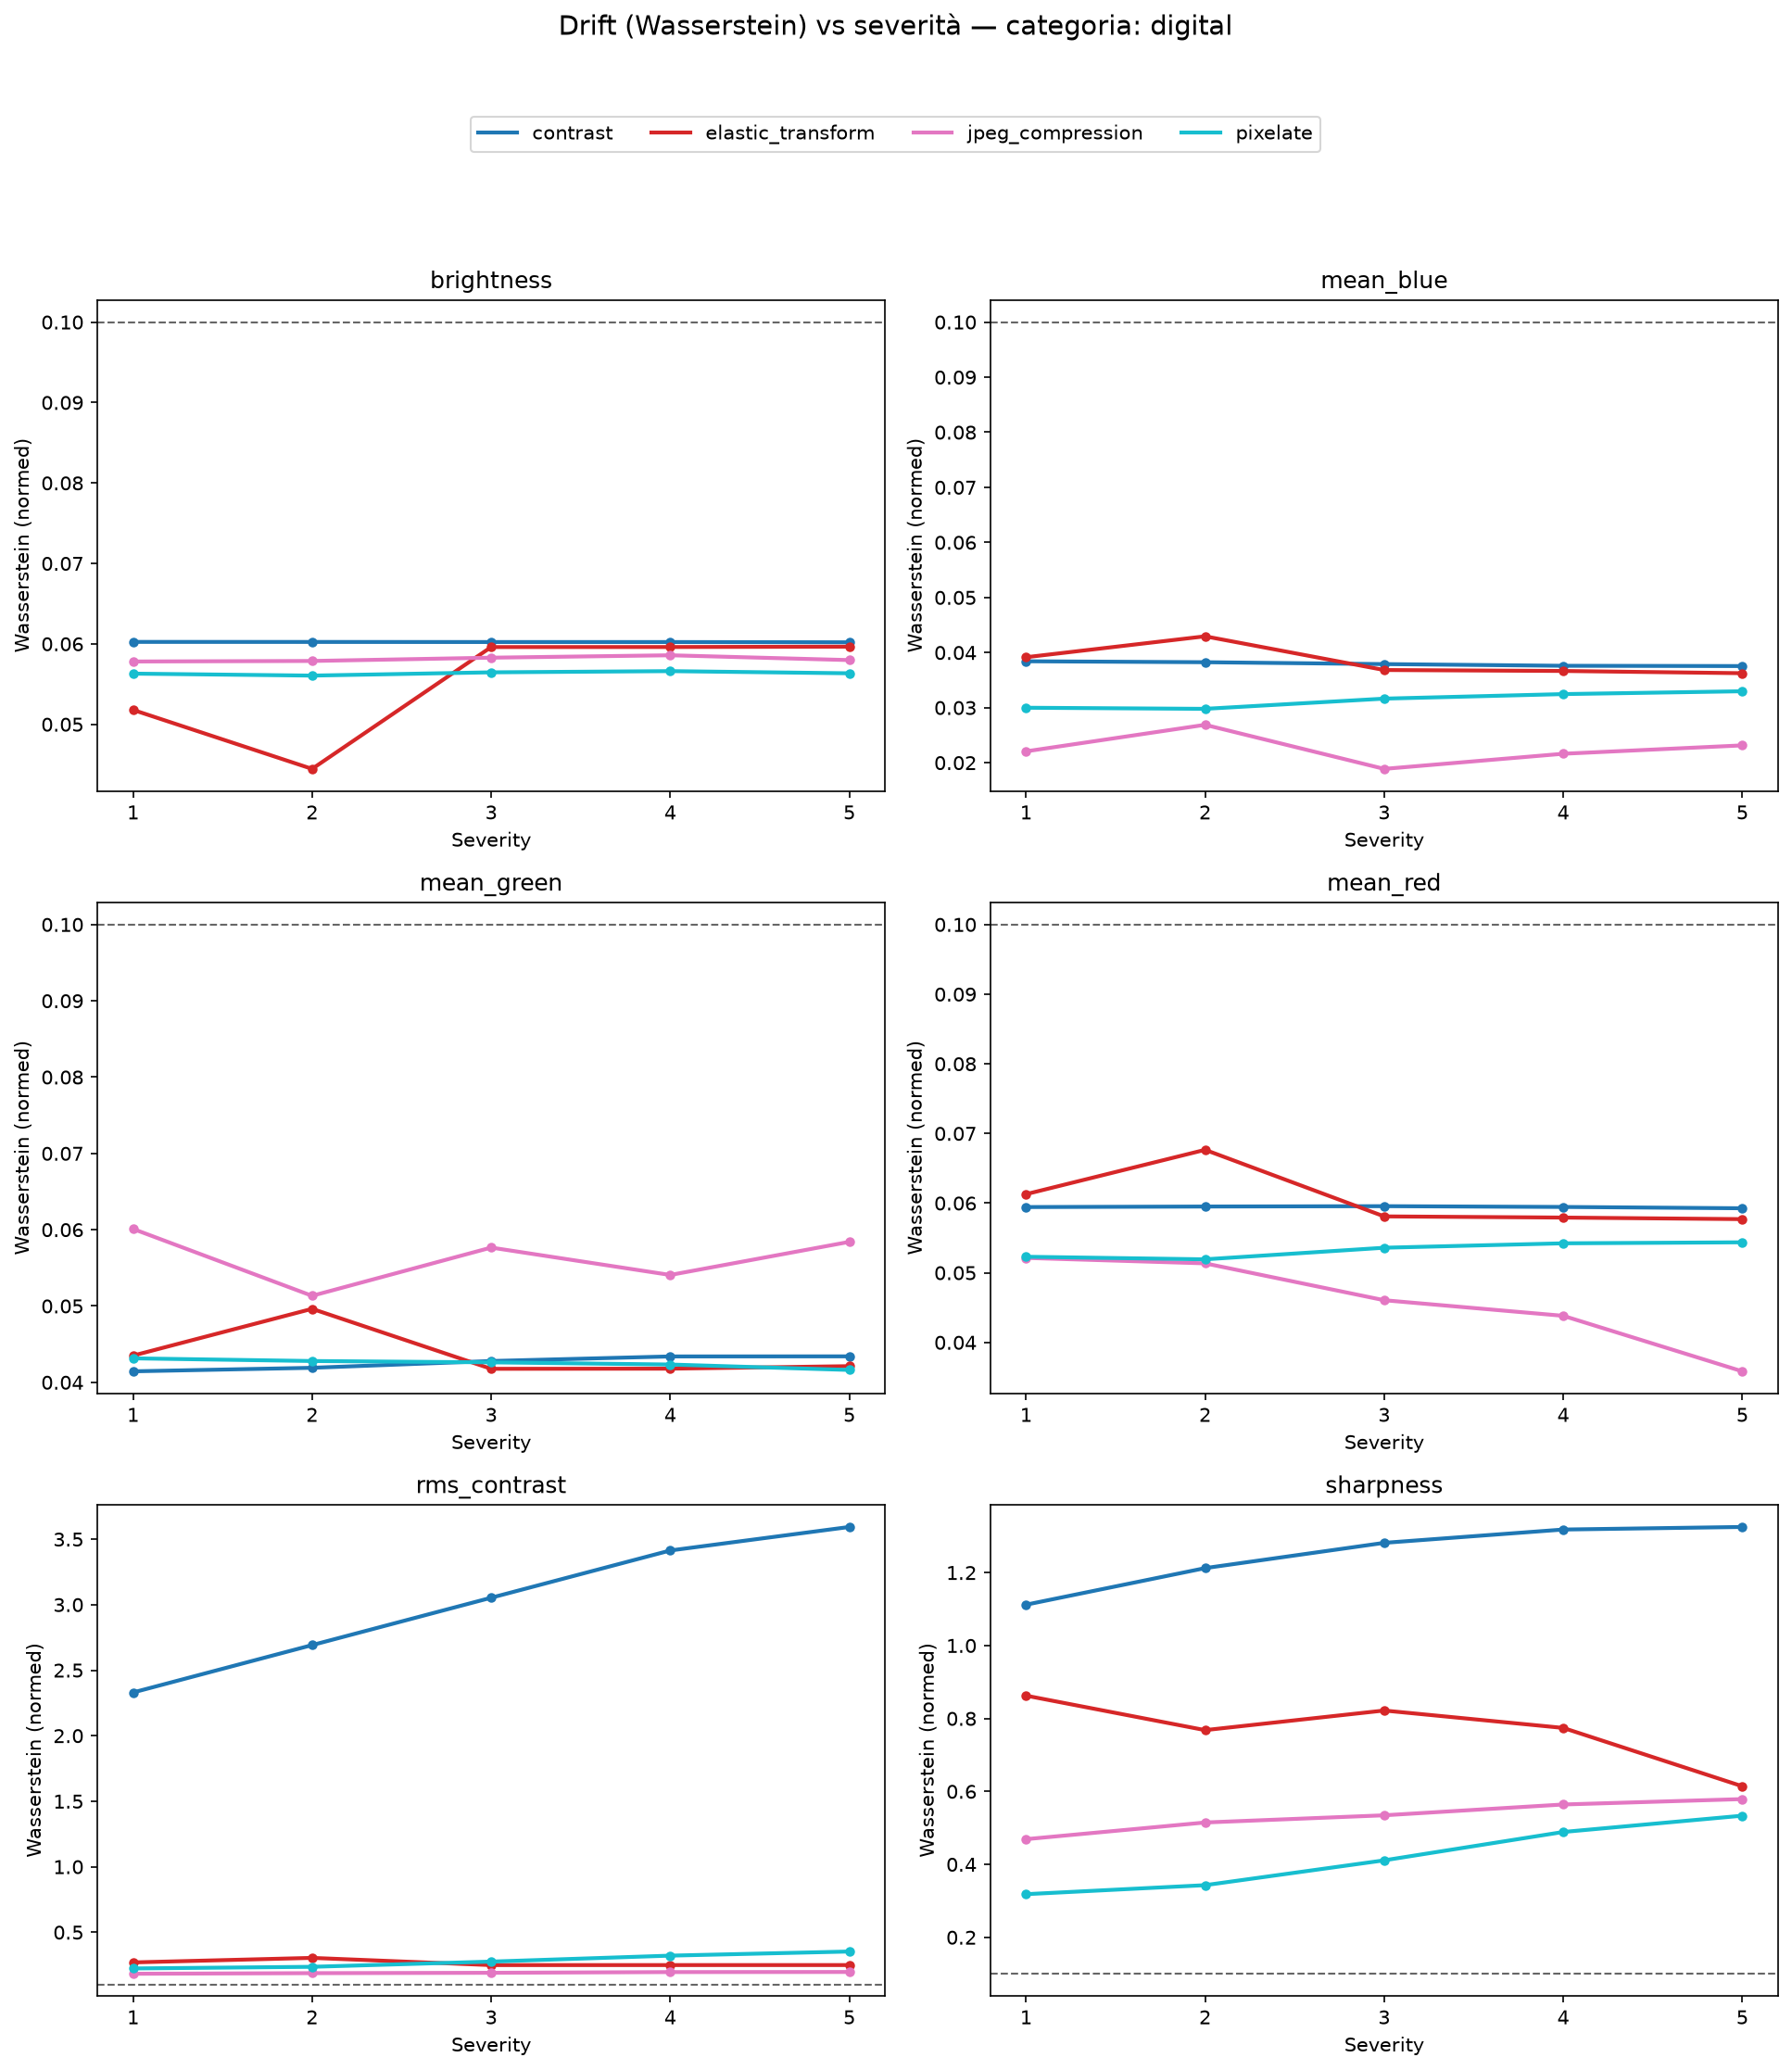
\includegraphics[width=\textwidth]{images/metrics/ImageNet-C/severity_curves/imagenet_c_severity_drift_digital.png}
	\caption{Distanza di Wesserstein tra le distribuzioni delle misure di luminanza, contrasto, nitidezza e media dei canali colore per ImageNet-C nel gruppo di corruzione digital, al variare della severità.}
	\label{fig:imagenet_c_drift_severity_digital}
\end{figure}
\begin{figure}[H]
	\centering
	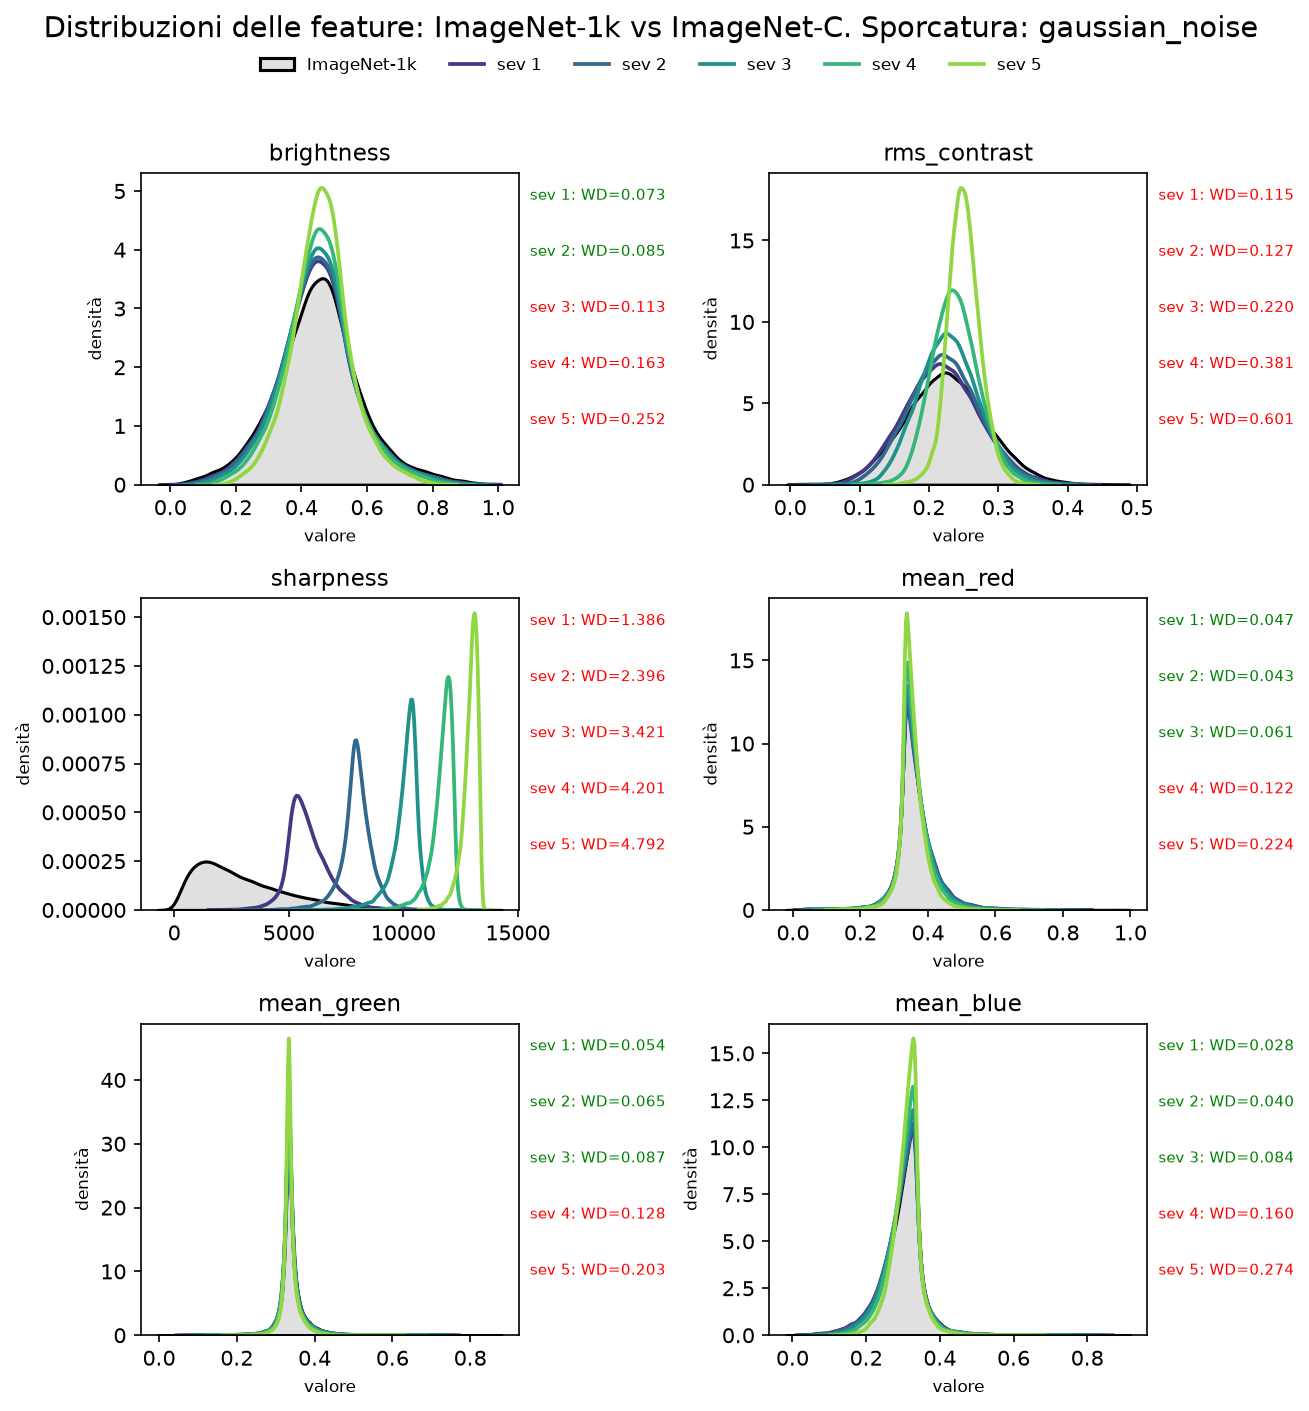
\includegraphics[width=\textwidth]{images/metrics/ImageNet-C/distributions_by_corruption/gaussian_noise.png}
	\caption{Distribuzione delle misure di luminanza, contrasto, nitidezza e media dei canali colore per ImageNet-1k e ImageNet-C con rumore gaussiano.}
	\label{fig:imagenet_c_drift_image_gaussian}
\end{figure}
\begin{figure}[H]
	\centering
	
\includegraphics[width=\textwidth]{images/metrics/ImageNet-C/distributions_by_corruption/shot_noise.png}
	\caption{Distribuzione delle misure di luminanza, contrasto, nitidezza e media dei canali colore per ImageNet-1k e ImageNet-C con rumore di shot.}
	\label{fig:imagenet_c_drift_image_shot}
\end{figure}
\begin{figure}[H]
	\centering
	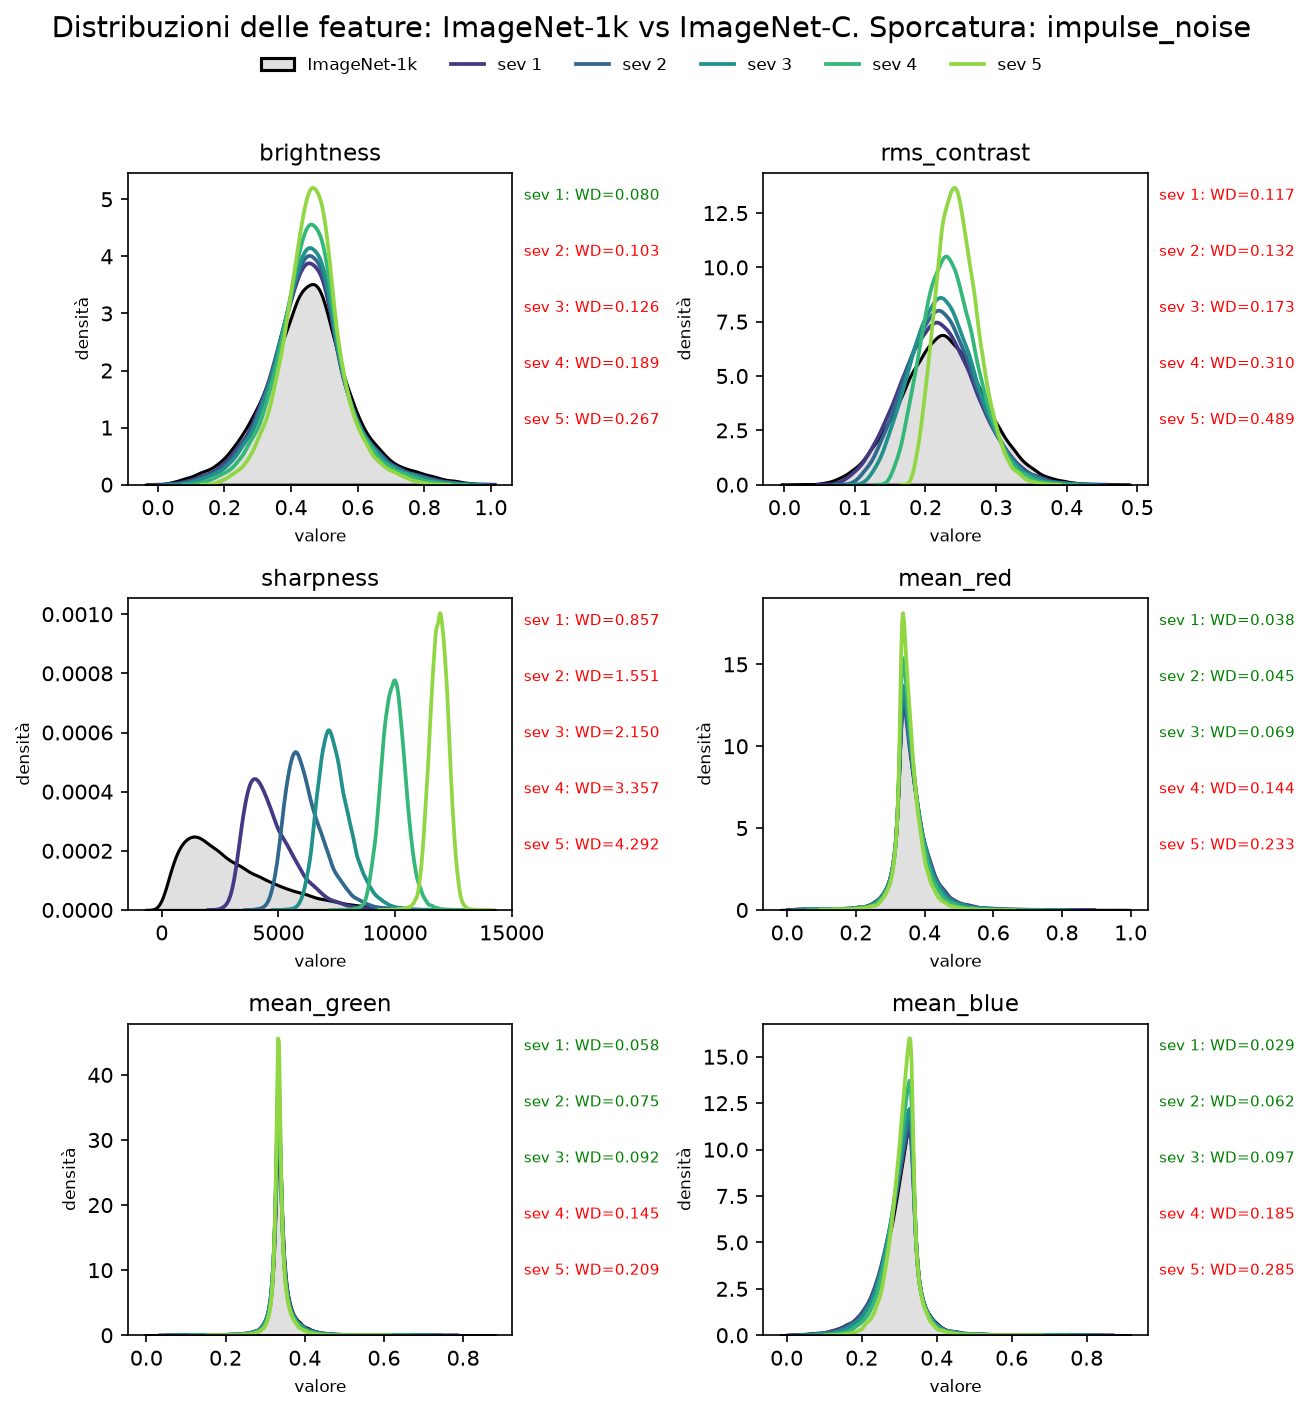
\includegraphics[width=\textwidth]{images/metrics/ImageNet-C/distributions_by_corruption/impulse_noise.png}
	\caption{Distribuzione delle misure di luminanza, contrasto, nitidezza e media dei canali colore per ImageNet-1k e ImageNet-C con rumore impulsivo.}
	\label{fig:imagenet_c_drift_image_impulse}
\end{figure}
\begin{figure}[H]
	\centering
	
\includegraphics[width=\textwidth]{images/metrics/ImageNet-C/distributions_by_corruption/defocus_blur.png}
	\caption{Distribuzione delle misure di luminanza, contrasto, nitidezza e media dei canali colore per ImageNet-1k e ImageNet-C con sfocatura da defocus.}
	\label{fig:imagenet_c_drift_image_defocus}
\end{figure}
\begin{figure}[H]
	\centering
	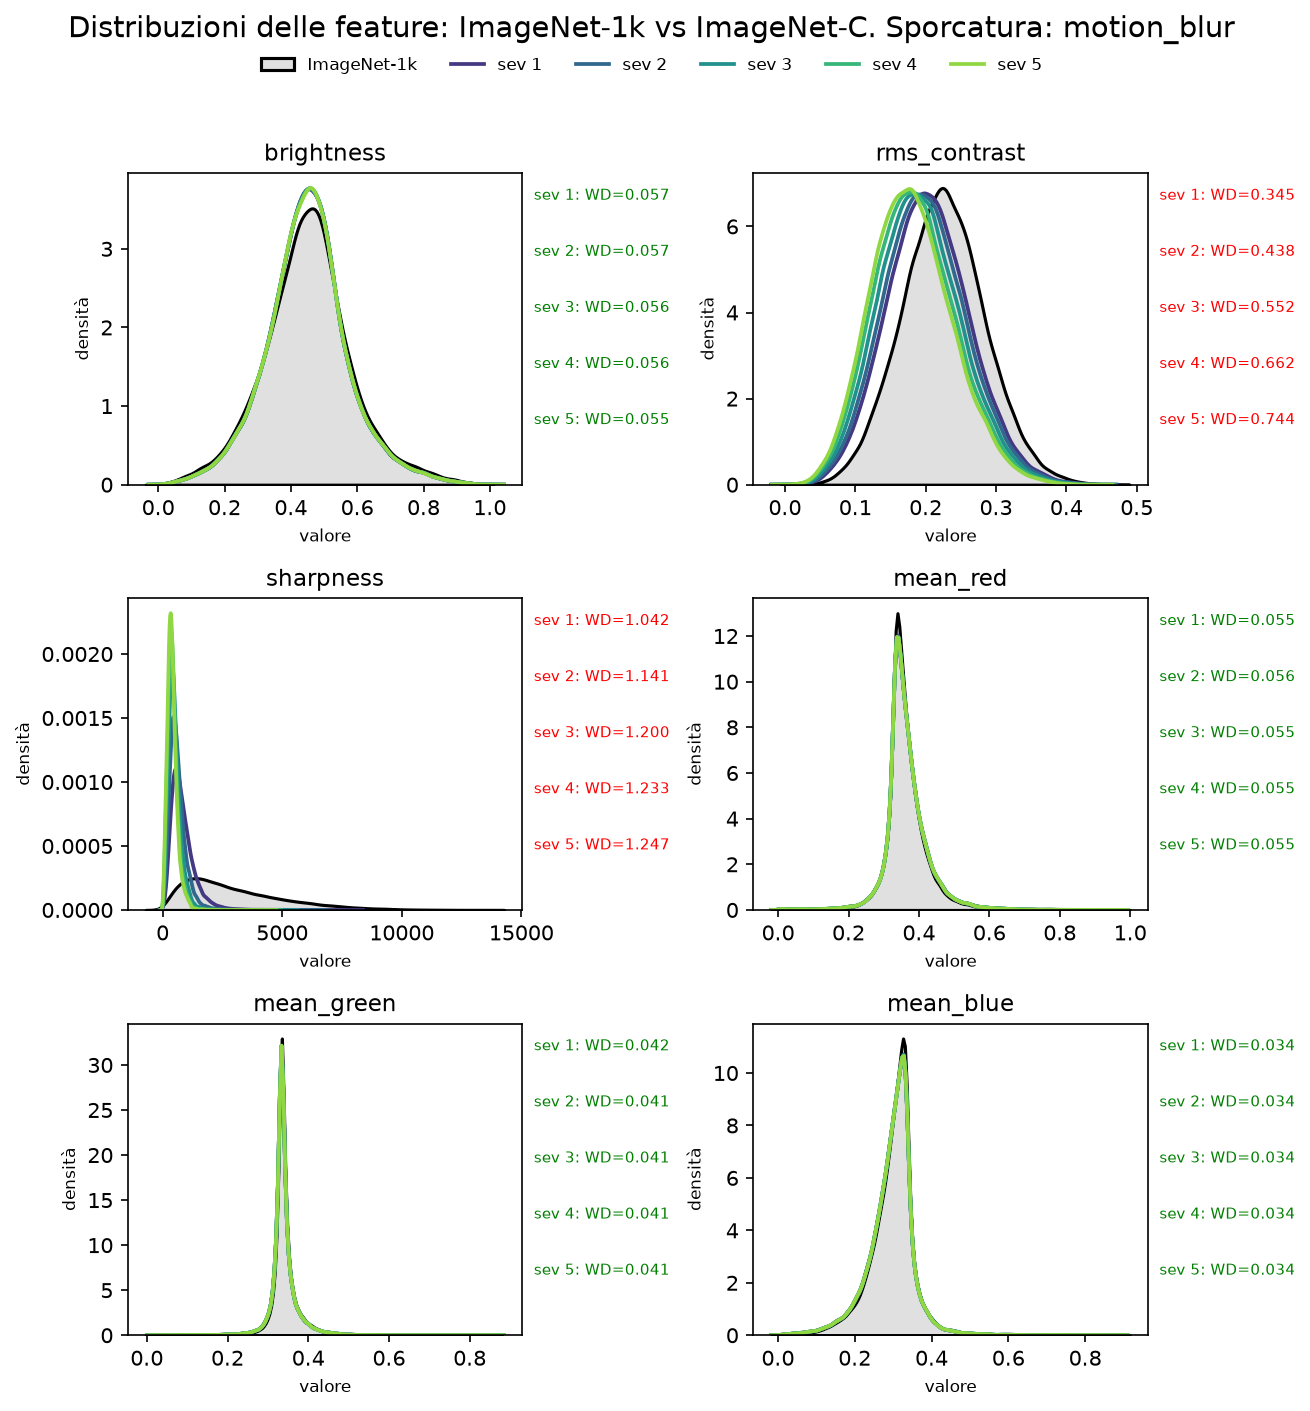
\includegraphics[width=\textwidth]{images/metrics/ImageNet-C/distributions_by_corruption/motion_blur.png}
	\caption{Distribuzione delle misure di luminanza, contrasto, nitidezza e media dei canali colore per ImageNet-1k e ImageNet-C con sfocatura da movimento.}
	\label{fig:imagenet_c_drift_image_motion}
\end{figure}
\begin{figure}[H]
	\centering
	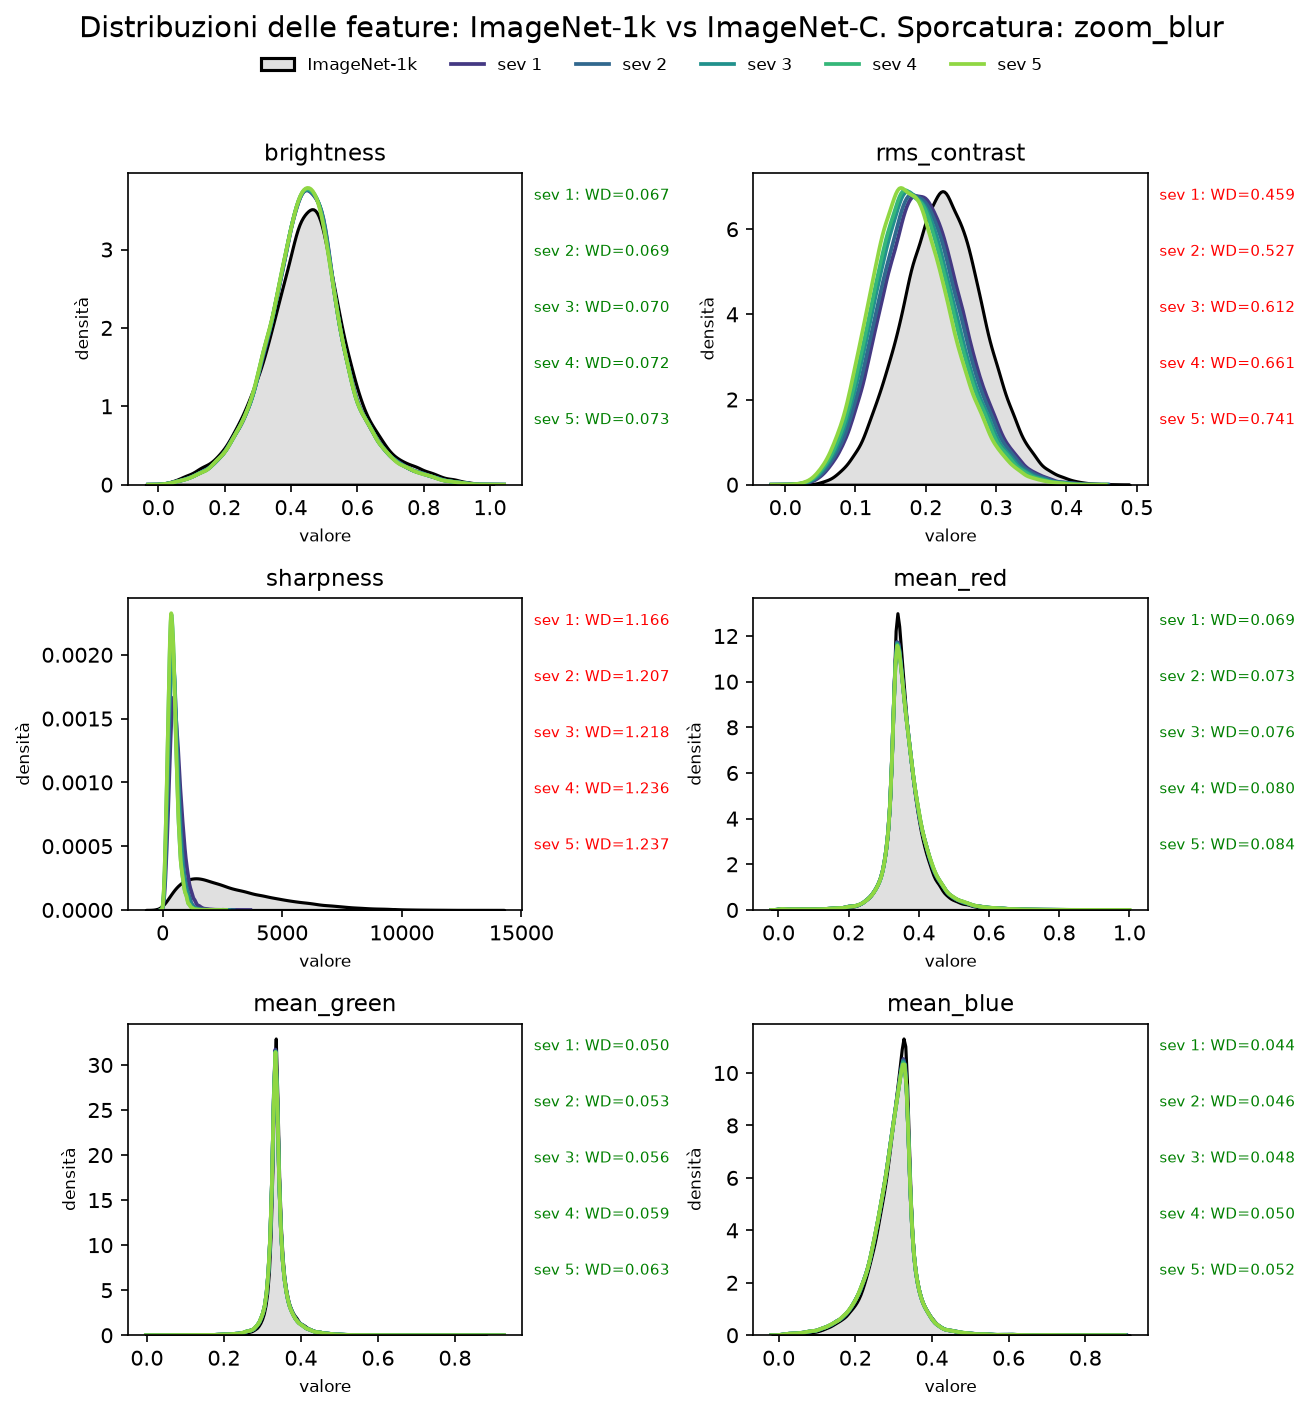
\includegraphics[width=\textwidth]{images/metrics/ImageNet-C/distributions_by_corruption/zoom_blur.png}
	\caption{Distribuzione delle misure di luminanza, contrasto, nitidezza e media dei canali colore per ImageNet-1k e ImageNet-C con sfocatura da zoom.}
	\label{fig:imagenet_c_drift_image_zoom}
\end{figure}
\begin{figure}[H]
	\centering
	
\includegraphics[width=\textwidth]{images/metrics/ImageNet-C/distributions_by_corruption/glass_blur.png}
	\caption{Distribuzione delle misure di luminanza, contrasto, nitidezza e media dei canali colore per ImageNet-1k e ImageNet-C con corruzione da vetro satinato.}
	\label{fig:imagenet_c_drift_image_glass}
\end{figure}
\begin{figure}[H]
	\centering
	
\includegraphics[width=\textwidth]{images/metrics/ImageNet-C/distributions_by_corruption/frost.png}
	\caption{Distribuzione delle misure di luminanza, contrasto, nitidezza e media dei canali colore per ImageNet-1k e ImageNet-C con corruzione da brina.}
	\label{fig:imagenet_c_drift_image_frost}
\end{figure}
\begin{figure}[H]
	\centering
	
\includegraphics[width=\textwidth]{images/metrics/ImageNet-C/distributions_by_corruption/fog.png}
	\caption{Distribuzione delle misure di luminanza, contrasto, nitidezza e media dei canali colore per ImageNet-1k e ImageNet-C con corruzione da nebbia.}
	\label{fig:imagenet_c_drift_image_fog}
\end{figure}
\begin{figure}[H]
	\centering
	
\includegraphics[width=\textwidth]{images/metrics/ImageNet-C/distributions_by_corruption/snow.png}
	\caption{Distribuzione delle misure di luminanza, contrasto, nitidezza e media dei canali colore per ImageNet-1k e ImageNet-C con corruzione da neve.}
	\label{fig:imagenet_c_drift_image_snow}
\end{figure}
\begin{figure}[H]
	\centering
	
\includegraphics[width=\textwidth]{images/metrics/ImageNet-C/distributions_by_corruption/brightness.png}
	\caption{Distribuzione delle misure di luminanza, contrasto, nitidezza e media dei canali colore per ImageNet-1k e ImageNet-C con corruzione da luminosità.}
	\label{fig:imagenet_c_drift_image_brightness}
\end{figure}
\begin{figure}[H]
	\centering
	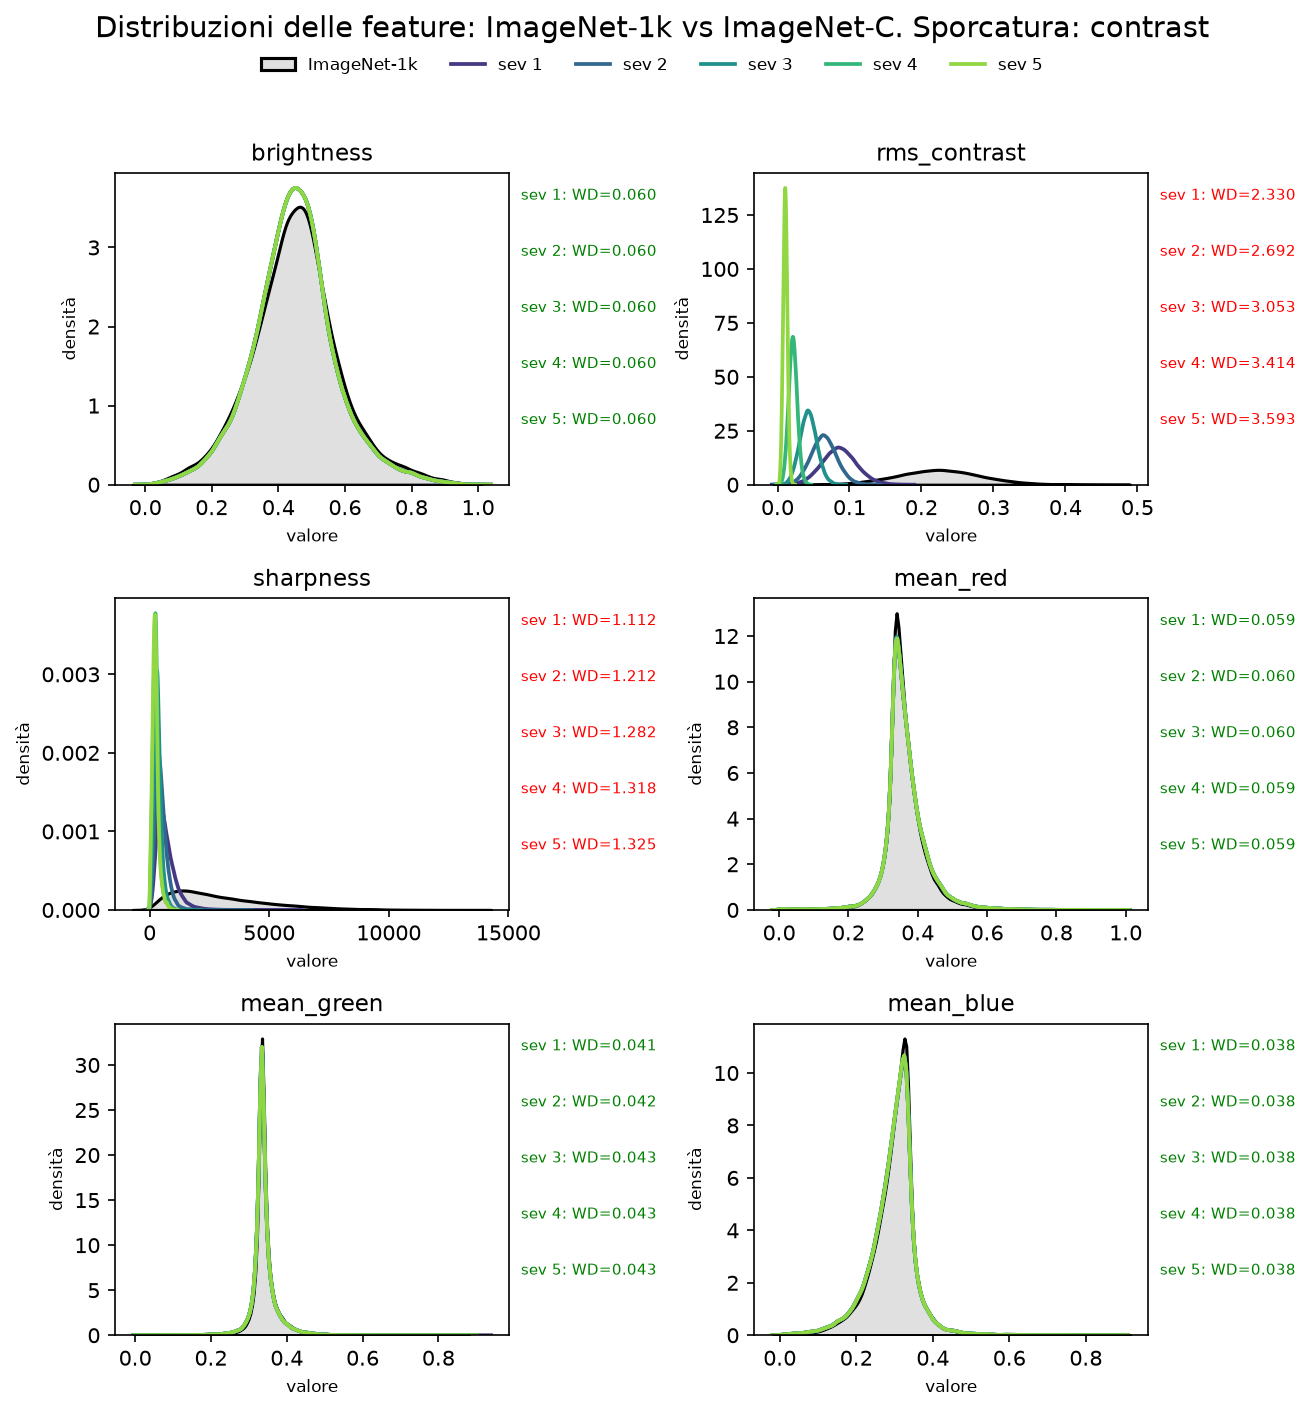
\includegraphics[width=\textwidth]{images/metrics/ImageNet-C/distributions_by_corruption/contrast.png}
	\caption{Distribuzione delle misure di luminanza, contrasto, nitidezza e media dei canali colore per ImageNet-1k e ImageNet-C con corruzione da contrasto.}
	\label{fig:imagenet_c_drift_image_contrast}
\end{figure}
\begin{figure}[H]
	\centering
	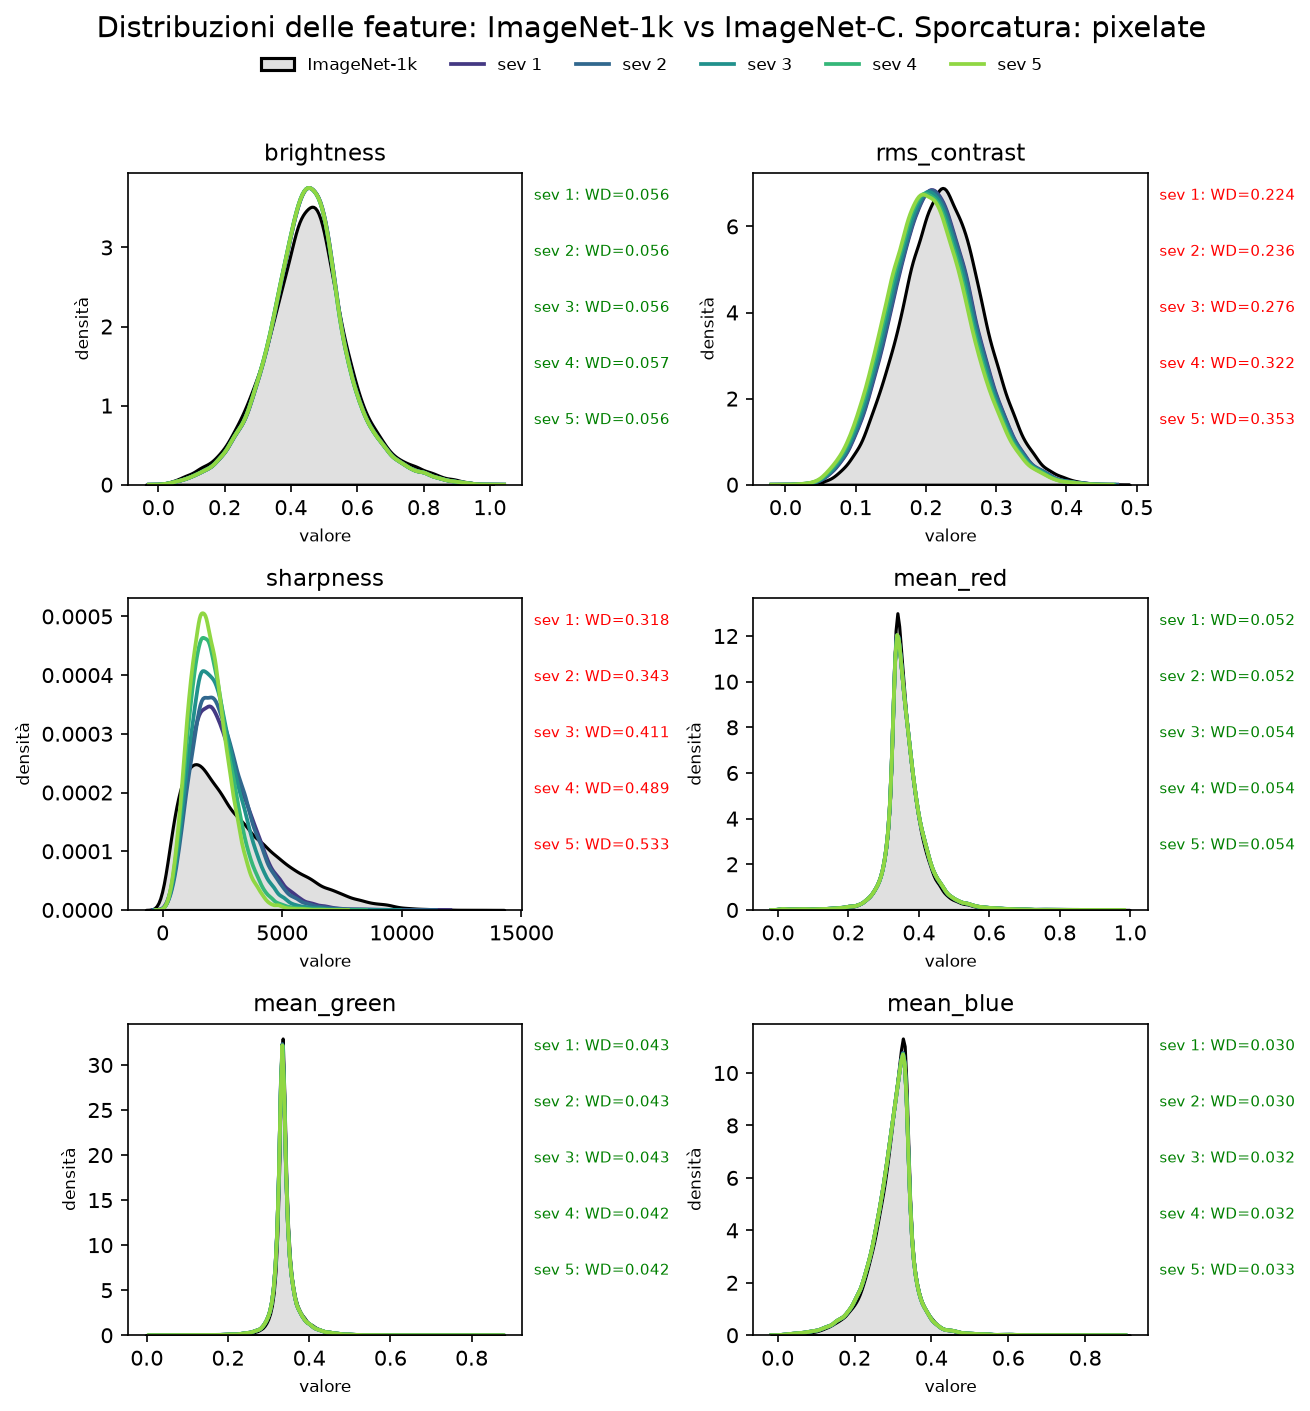
\includegraphics[width=\textwidth]{images/metrics/ImageNet-C/distributions_by_corruption/pixelate.png}
	\caption{Distribuzione delle misure di luminanza, contrasto, nitidezza e media dei canali colore per ImageNet-1k e ImageNet-C con corruzione da pixelizzazione.}
	\label{fig:imagenet_c_drift_image_pixelate}
\end{figure}
\begin{figure}[H]
	\centering
	
\includegraphics[width=\textwidth]{images/metrics/ImageNet-C/distributions_by_corruption/jpeg_compression.png}
	\caption{Distribuzione delle misure di luminanza, contrasto, nitidezza e media dei canali colore per ImageNet-1k e ImageNet-C con corruzione da compressione JPEG.}
	\label{fig:imagenet_c_drift_image_jpeg}
\end{figure}
\begin{figure}[H]
	\centering
	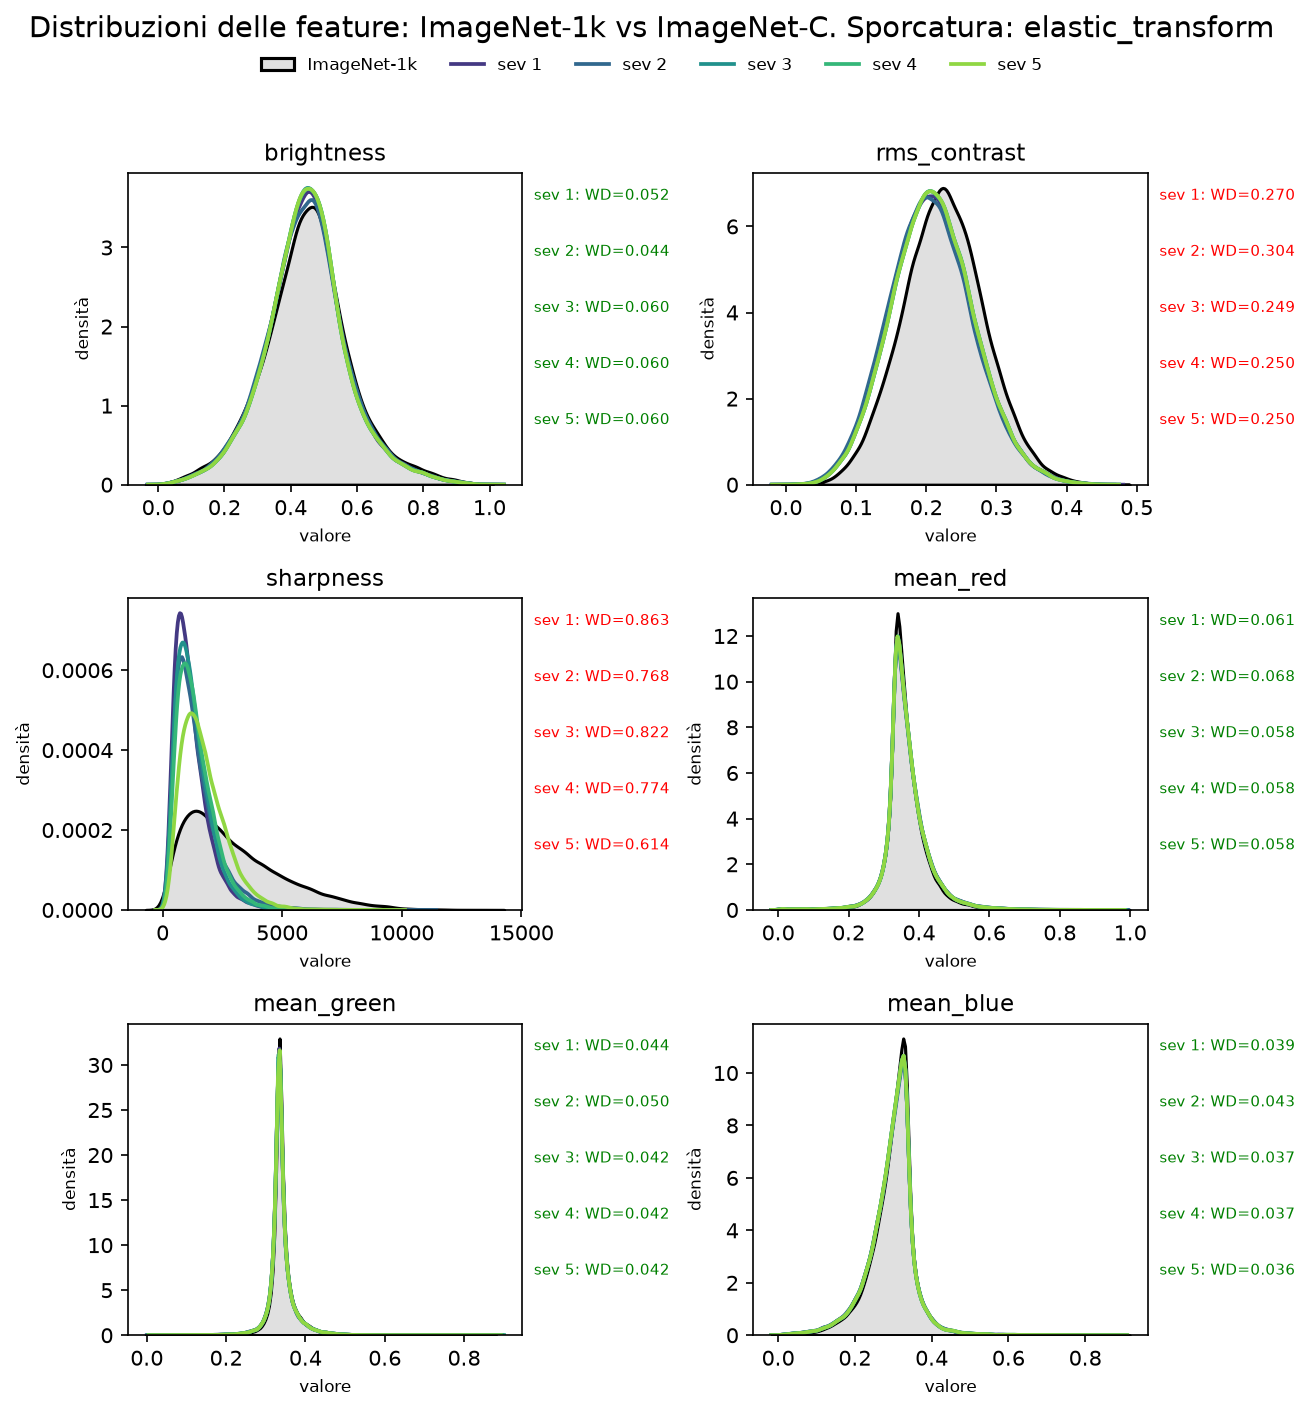
\includegraphics[width=\textwidth]{images/metrics/ImageNet-C/distributions_by_corruption/elastic_transform.png}
	\caption{Distribuzione delle misure di luminanza, contrasto, nitidezza e media dei canali colore per ImageNet-1k e ImageNet-C con corruzione da trasformazione elastica.}
	\label{fig:imagenet_c_drift_image_elastic}
\end{figure}
\section{Analisi delle metriche di drift sulle feature del modello}
In questa sezione vengono analizzate le metriche di drift calcolate sulle feature del modello ResNet-50, estratte dal layer \texttt{avgpool}. Come già accennato nella sezione 4, la rilevazione delle feature viene effettuata tramite test MMD.I test sono stati effettuati con un valore di soglia uguale a $0.05$, quindi viene rilevato un drift quando il p-value $p < 0.05$
\subsection{ImageNet-1k vs ImageNet-R}
Il test MMD ImageNet-R è stato effettuato rispetto alle feature ottenute dalla classificazione di ImageNet-1k sottocampionato alle duecento classi in comune con ImageNet-R.
\begin{table}[H]
  \centering
  \begin{tabular}{llll}
    \toprule
    dataset & is\_drift & p\_val & distance \\
    \midrule
    ImageNetR & True & 0.0000 & 0.0805 \\ 
    \bottomrule
  \end{tabular}
	\caption{Risultati del test di MMD tra le feature estratte dal layer \texttt{avgpool} del modello ResNet-50 per ImageNet-1k e ImageNet-R.}
	\label{tab:mmd_drift_report}
\end{table}
Come si può notare dal risultato riportato in tabella \ref{tab:mmd_drift_report}, il p-value del test è zero, quindi al di sotto della soglia di rilevazione. La rilevazione del drift è quindi coerente con il drift rilevato per le feature visive, come si può
vedere in figura \ref{fig:imagenet_r_drift_image}.
\subsection{ImageNet-1k vs ImageNet-C}
Per poter fare l'analisi di MMD delle feature, è stato necessario effettuare un campionamento a 10.000 esempi, in quanto utilizzare l'intero dataset avrebbe richiesto una quantità di memoria della GPU a noi non disponibile. Il campionamento è casuale, mantenendo un numero equo di esempi per ogni classe. 

Analizziamo ora le metriche di drift rilevate nelle feature utilizzate dal modello durante la classificazione e confrontiamo il risultato con il drift rilevato nelle feature visive.
\subsubsection{Blur}
\begin{table}[H]
  \centering
  \begin{tabular}{lllll}
    \toprule
    corruption & severity & is\_drift & p\_val & distance \\
    \midrule
    defocus\_blur & 1 & True & 0.0000 & 0.0002 \\ 
    defocus\_blur & 2 & True & 0.0000 & 0.0003 \\ 
    defocus\_blur & 3 & True & 0.0000 & 0.0005 \\ 
    defocus\_blur & 4 & True & 0.0000 & 0.0009 \\ 
    defocus\_blur & 5 & True & 0.0000 & 0.0022 \\ 
    glass\_blur & 1 & True & 0.0000 & 0.0002 \\ 
    glass\_blur & 2 & True & 0.0000 & 0.0031 \\ 
    glass\_blur & 3 & True & 0.0000 & 0.0176 \\ 
    glass\_blur & 4 & True & 0.0000 & 0.0321 \\ 
    glass\_blur & 5 & True & 0.0000 & 0.0238 \\ 
    motion\_blur & 1 & False & 0.2000 & 0.0000 \\ 
    motion\_blur & 2 & False & 0.1500 & 0.0001 \\ 
    motion\_blur & 3 & True & 0.0000 & 0.0013 \\ 
    motion\_blur & 4 & True & 0.0000 & 0.0099 \\ 
    motion\_blur & 5 & True & 0.0000 & 0.0229 \\ 
    zoom\_blur & 1 & True & 0.0000 & 0.0006 \\ 
    zoom\_blur & 2 & True & 0.0000 & 0.0021 \\ 
    zoom\_blur & 3 & True & 0.0000 & 0.0017 \\ 
    zoom\_blur & 4 & True & 0.0000 & 0.0027 \\ 
    zoom\_blur & 5 & True & 0.0000 & 0.0013 \\ 
    \bottomrule
  \end{tabular}
\caption{Risultati del test di MMD tra le feature estratte dal layer \texttt{avgpool} del modello ResNet-50 per ImageNet-1k e ImageNet-C, corruzione di tipo blur.}
\label{tab:mmd_drift_report_imagenet_c_blur}
\end{table}
Per quanto riguarda la classe di sporcature blur, abbiamo ottenuto i risultati presentati in tabella \ref{tab:mmd_drift_report_imagenet_c_blur}. Possiamo effettuare le seguenti osservazioni:
\begin{itemize}
  \item \textbf{defocus\_blur}: Il drift viene rilevato ad ogni livello di severity; il ché è coerente con il drift rilevato nelle feature visive, come presentato in figura \ref{fig:imagenet_c_drift_image_defocus}. Infatti, in questo tipo di sporcatura sharpness e rms\_contrast presentano un drift a tutti i livelli di severity.
  \item \textbf{glass\_blur}: Come si può notare in figura \ref{fig:imagenet_c_drift_image_glass}, le feature sharpness e rms\_contrast presentano un drift a tutti i livelli di severity. Valgono quindi le stesse considerazioni effettuate per defocus\_blur.
  \item \textbf{motion\_blur}: Nonostante venga rilevato, come nelle due sporcature precedenti e riportato in figura \ref{fig:imagenet_c_drift_image_motion}, un drift nelle feature sharpness e rms\_contrast in tutti di livelli di severità, con distanze di Wesserstein simili a quelle rilevate per defocus\_blur e glass\_blur, le feature estratte dal modello per i primi due livelli non presentano drift rispetto alle feature estratte da ImageNet-1k. Infatti, le feature che il modello estrae e utilizza per la classificazione sono fondamentalmente diverse rispetto a quelle estraibili direttamente dalle immagini, quindi è possibile che, nonostante la sporcatura, le feature estratte per i primi due livelli di severità non presentino drift rispetto a quelle estratte per imagenet-1k.
  \item \textbf{zoom\_blur}: Valgono le stesse considerazioni effettuate per defocus\_blur e glass\_blur. Ciò si può notare osservando la figura \ref{fig:imagenet_c_drift_image_zoom}.
\end{itemize}
\subsubsection{Digital}

\begin{table}[H]
  \centering
  \begin{tabular}{lllll}
    \toprule
    corruption & severity & is\_drift & p\_val & distance \\
    \midrule
    contrast & 1 & False & 0.2500 & 0.0000 \\ 
    contrast & 2 & False & 0.1500 & 0.0001 \\ 
    contrast & 3 & False & 0.1500 & 0.0001 \\ 
    contrast & 4 & True & 0.0000 & 0.0005 \\ 
    contrast & 5 & True & 0.0000 & 0.0029 \\ 
    elastic\_transform & 1 & False & 0.2500 & 0.0001 \\ 
    elastic\_transform & 2 & True & 0.0000 & 0.0011 \\ 
    elastic\_transform & 3 & True & 0.0000 & 0.0017 \\ 
    elastic\_transform & 4 & True & 0.0000 & 0.0083 \\ 
    elastic\_transform & 5 & True & 0.0000 & 0.0740 \\ 
    jpeg\_compression & 1 & False & 0.0500 & 0.0001 \\ 
    jpeg\_compression & 2 & False & 0.1500 & 0.0001 \\ 
    jpeg\_compression & 3 & False & 0.1000 & 0.0002 \\ 
    jpeg\_compression & 4 & False & 0.0500 & 0.0002 \\ 
    jpeg\_compression & 5 & False & 0.0500 & 0.0002 \\ 
    pixelate & 1 & False & 0.2000 & 0.0001 \\ 
    pixelate & 2 & True & 0.0000 & 0.0002 \\ 
    pixelate & 3 & True & 0.0000 & 0.0005 \\ 
    pixelate & 4 & True & 0.0000 & 0.0020 \\ 
    pixelate & 5 & True & 0.0000 & 0.0126 \\ 
    \bottomrule
  \end{tabular}
\caption{Risultati del test di MMD tra le feature estratte dal layer \texttt{avgpool} del modello ResNet-50 per ImageNet-1k e ImageNet-C, corruzione di tipo digital.}
\label{tab:mmd_drift_report_imagenet_c_digital}
\end{table}
Per quanto riguarda la classe di sporcature digital, abbiamo ottenuto i risultati presentati in tabella \ref{tab:mmd_drift_report_imagenet_c_digital}. Possiamo effettuare le seguenti osservazioni:
\begin{itemize}
  \item \textbf{contrast}: A differenza di quanto rilevato per le feature visive rms\_contrast e sharpness, come si può vedere in figura \ref{fig:imagenet_c_drift_image_contrast}, il test MMD non rileva una presenza di drift nelle feature ai primi tre livello di severità. Valgono quindi le stesse considerazioni effettuate per motion\_blur.
  \item \textbf{eleastic\_transform}: Come rilevato per contrast, vi è una discrepanza fra il drift rilevato nelle feature visive, riportato in figura \ref{fig:imagenet_c_drift_image_elastic}, e il drift rilevato nelle feature estratte dal modello. In particolare, esse non risultano soggette a drift per il primo livello di severity.
  \item \textbf{jpeg\_compression}: Per questo tipo di sporcatura, le feature estratte dal modello non risultano soggette a drift per nessun livello di severity, nonostante le feature visive rms\_contrast e sharpness risultino soggette a drift, seppur con distanza di Wesserstein più bassa rispetto ad altri tipi di sporcatura. Ciò è riportato in figura \ref{fig:imagenet_c_drift_image_jpeg}. Questo è dato probabilmente dal fatto che le feature estratte per questo tipo di sporcature presentino un drift minimo o nullo rispetto alle feature di riferimento.
  \item \textbf{pixelate}: A differenza di quanto rilevato per le feature visive rms\_contrast e sharpness, riportato in figura \ref{fig:imagenet_c_drift_image_pixelate}, le feature estratte dal modello presentano drift solo nel primo livello di severity. Valgono quindi le considerazioni fatte in precedenza.
\end{itemize}
\subsubsection{Noise}
\begin{table}[H]
  \centering
  \begin{tabular}{lllll}
    \toprule
    corruption & severity & is\_drift & p\_val & distance \\
    \midrule
    gaussian\_noise & 1 & False & 0.5000 & 0.0000 \\ 
    gaussian\_noise & 2 & True & 0.0000 & 0.0005 \\ 
    gaussian\_noise & 3 & True & 0.0000 & 0.0025 \\ 
    gaussian\_noise & 4 & True & 0.0000 & 0.0110 \\ 
    gaussian\_noise & 5 & True & 0.0000 & 0.0682 \\ 
    impulse\_noise & 1 & True & 0.0000 & 0.0004 \\ 
    impulse\_noise & 2 & True & 0.0000 & 0.0014 \\ 
    impulse\_noise & 3 & True & 0.0000 & 0.0040 \\ 
    impulse\_noise & 4 & True & 0.0000 & 0.0215 \\ 
    impulse\_noise & 5 & True & 0.0000 & 0.0840 \\ 
    shot\_noise & 1 & False & 0.2000 & 0.0000 \\ 
    shot\_noise & 2 & True & 0.0000 & 0.0005 \\ 
    shot\_noise & 3 & True & 0.0000 & 0.0028 \\ 
    shot\_noise & 4 & True & 0.0000 & 0.0155 \\ 
    shot\_noise & 5 & True & 0.0000 & 0.0433 \\ 
    \bottomrule
  \end{tabular}
\caption{Risultati del test di MMD tra le feature estratte dal layer \texttt{avgpool} del modello ResNet-50 per ImageNet-1k e ImageNet-C, corruzione di tipo noise.}
\label{tab:mmd_drift_report_imagenet_c_noise}
\end{table}
Per quanto riguarda la classe di sporcature noise, abbiamo ottenuto i risultati presentati in tabella \ref{tab:mmd_drift_report_imagenet_c_noise}. Possiamo effettuare le seguenti osservazioni:
\begin{itemize}
  \item \textbf{gaussian\_noise}: Per questo tipo di sporcatura, le feature visive rms\_contrast, sharpness presentano sempre un drift, le medie dei canali colore presentano un drift dal quarto livello di severità in poi e brightness presenta un drift dal terzo livello di severità in poi. Questi risultati sono riportati in figura \ref{fig:imagenet_c_drift_image_gaussian}. A differenza di quanto rilevato nelle feature visive, le feature estratte dal modello presentano un drift solamente dal secondo livello di severità. Come quindi già detto in precedenza, le feature estratte dal modello per il primo livello di severità sono uguali a quelle estratte per ImageNet-1k, infatti la distanza MMD rilevata è $0$.
  \item \textbf{impulse\_noise}: Per questo tipo di sporcatura, le feature visive rms\_contrast e sharpness presentano sempre un drift, le medie dei canali colore presentano un drift dal quarto livello di severità e brightness dal secondo livello di severità. Ciò è riportato nella figura \ref{fig:imagenet_c_drift_image_impulse}. Come rilevato in precedenza, vi è quindi una discrepanza tra il drift rilevato nelle feature visive e quello rilevato nelle feature estratte dal modello: infatti, quest'ultime presentano sempre un drift rispetto alle feature di riferimento.
  \item \textbf{shot\_noise}: Per questo tipo di sporcatura, le feature visive rms\_contrast e sharpness presentano sempre un drift, brightness presenta un drift dal terzo livello di severità in poi. A differenza degli altri tipi di sporcatura in questa classe, l'unica media del canale colore che presenta un drift è quella del canale blu all'ultimo livello di severity.
  Anche in questo caso, il drift rilevato nelle feature estratte dal modello diverge rispetto a quanto rilevato nelle feature visive: infatti, viene rilevato un drift solamente dal secondo livello di severità. 
\end{itemize}
\subsubsection{Weather}
\begin{table}[H]
  \centering
  \begin{tabular}{lllll}
    \toprule
    corruption & severity & is\_drift & p\_val & distance \\
    \midrule
    brightness & 1 & False & 0.3500 & 0.0000 \\ 
    brightness & 2 & False & 0.1000 & 0.0001 \\ 
    brightness & 3 & False & 0.1000 & 0.0000 \\ 
    brightness & 4 & False & 0.2500 & 0.0001 \\ 
    brightness & 5 & True & 0.0000 & 0.0003 \\ 
    fog & 1 & False & 0.3500 & 0.0000 \\ 
    fog & 2 & False & 0.1500 & 0.0001 \\ 
    fog & 3 & False & 0.2500 & 0.0001 \\ 
    fog & 4 & False & 0.1000 & 0.0002 \\ 
    fog & 5 & True & 0.0000 & 0.0021 \\ 
    frost & 1 & False & 0.1500 & 0.0000 \\ 
    frost & 2 & True & 0.0000 & 0.0004 \\ 
    frost & 3 & True & 0.0000 & 0.0016 \\ 
    frost & 4 & True & 0.0000 & 0.0020 \\ 
    frost & 5 & True & 0.0000 & 0.0043 \\ 
    snow & 1 & True & 0.0000 & 0.0003 \\ 
    snow & 2 & True & 0.0000 & 0.0010 \\ 
    snow & 3 & True & 0.0000 & 0.0032 \\ 
    snow & 4 & True & 0.0000 & 0.0050 \\ 
    snow & 5 & True & 0.0000 & 0.0133 \\ 
    \bottomrule
  \end{tabular}
\caption{Risultati del test di MMD tra le feature estratte dal layer \texttt{avgpool} del modello ResNet-50 per ImageNet-1k e ImageNet-C, corruzione di tipo weather.}
\label{tab:mmd_drift_report_imagenet_c_weather}
\end{table}
Per quanto riguarda la classe di sporcature weather, abbiamo ottenuto i risultati presentati in tabella \ref{tab:mmd_drift_report_imagenet_c_weather}. Possiamo effettuare le seguenti osservazioni:
\begin{itemize}
  \item \textbf{brightness}: Per questo tipo di sporcatura, si presenta un drift in tutte le feature visive e a tutti i livelli di severity tranne per le medie dei canali colore, le quali non presentano alcun tipo di drift. Ciò è riportato in figura \ref{fig:imagenet_c_drift_image_brightness}. Come si può osservare dalla tabella \ref{tab:mmd_drift_report_imagenet_c_weather}, le feature estratte dal modello presentano un drift rispetto a quelle estratte da ImageNet-1k solamente al quinto livello di severity. Valgono quindi le considerazioni effettuate in precedenza sulle feature estratte dal modello.
  \item \textbf{fog}: Per questo tipo di sporcatura, tutte le feature visive presentano un drift a tutti i livelli di severità. La figura \ref{fig:imagenet_c_drift_image_fog} presenta il drift misurato su queste feature. Ciò non si riflette nelle feature estratte dal modello, nelle quali viene rilevato un drift dal test MMD solamente al quinti livello di severità.
  \item \textbf{frost}: Per questo tipo di sporcatura, tutte le feature visive presentano un drift a tutti i livelli di severità. La figura \ref{fig:imagenet_c_drift_image_frost} presenta il drift misurato su queste feature. Ciò si riflette solamente parzialmente sulle feature estratte dal modello: infatti, viene rilevato un drift in esse solamente dal secondo livello di severità.
  \item \textbf{snow}: Per questo tipo di sporcatura, tutte le feature visive presentano un drift a tutti i livelli di severità tranne rms\_contrast, la quale presenta un drift solamente a partire dal secondo livello di severità. La figura \ref{fig:imagenet_c_drift_image_snow} presenta il drift misurato su queste feature. Ciò si riflette quindi solamente parzialmente sulle feature estratte dal modello: infatti, viene rilevato un drift in esse a tutti i livelli di severità.
\end{itemize}
\subsubsection{Analisi del confronto tra tipi di feature}
Confrontando i risultati ottenuti per la rilevazione del drift sulle feature visive e sulle feature estratte dal modello, si può evincere che non vi è una correlazione diretta tra la presenza di drift nelle due. Ciò può essere dato dal fatto che la rete convolutiva computa e utilizza feature map le quali non sono direttamente confrontabili con le feature visive direttamente estratte dall'immagine, nonostante esse possano venir utilizzate per calcolare le feature map. Il drift delle feature del modello non sembra quindi essere influenzato dal drift nelle feature visive.
\section{Analisi delle performance del modello}
In questa sezione vengono analizzate le performance del modello ResNet-50 su ImageNet-R e ImageNet-C. Per ImageNet-R, confronteremo le metriche ottenute dalla classificazione delle immagini del dataset con le metriche ottenute dalla classificazione delle immagini di ImageNet-1k. Per ImageNet-C, invece, analizzeremo l'accuracy del modello al variare della severità della corruzione, calcolando la degradazione delle performance rispetto alla severity, calcolando la robustezza del modello e misurando quanto linearmente la severità della corruzione influisca sulla degradazione delle performance del modello.
\subsection{ImageNet-1k vs ImageNet-R}

\subsection{ImageNet-1k vs ImageNet-C}